\documentclass[10pt,a4paper]{article}

%double si on veut une version prof et une version élève. simple si on veut une seule version.
\newcommand{\buildmode}{double}

\InputIfFileExists{version.tex}{}{}
% Version (définie par le script)
\providecommand{\version}{eleve}

\usepackage{feuilleexo}

%%%à modifier à chaque fois

\renewcommand{\niveau}{1G}
\renewcommand{\chapitre}{Probabilités conditionnelles}
\renewcommand{\numchap}{2}
\renewcommand{\theme}{Probabilités}

\begin{document}




%\legendeicones

\vspace{-0.3cm}

\begin{prerequis}
\begin{itemize}
    \item Univers \(\Omega\) d'une expérience aléatoire, loi de probabilité.
    \item Évènement, évènement contraire \(\overline{A}\).
    \item Réunion \(A\cup B\) et intersection \(A\cap B\) de deux évènements.
    \item Résoudre une équation du premier degré.
\end{itemize}
\end{prerequis}

\begin{multicols}{2}

\section{Bilan de probabilités (rappels de Seconde)}

\begin{exo}
On lance un dé à douze faces numérotées de 1 à 12.
On considère les événements :
\begin{itemize}
    \item $A$: « on obtient un diviseur de 12» ;
    \item $B$: « on obtient un multiple de 3» ;
    \item $C$: « on obtient un nombre premier ».
\end{itemize}

\begin{enumerate}
    \item Proposer un univers et une loi de probabilité adaptés à la situation.
    \item Écrire les évènements $A$, $B$ et $C$ sous forme d'ensemble.
    \item Déterminer $P(A)$.
    \item Donner l'écriture ensembliste de l'événement\\ $A \cap B$ et en déduire sa probabilité.
    \item Donner l'écriture ensembliste de l'événement\\ $A \cup C$ et en déduire sa probabilité.
    \item Donner l'écriture ensembliste de l'événement\\ $\overline{B} $ et en déduire sa probabilité.
\end{enumerate}
\end{exo}


\prof{
\begin{itemize}
    \item \(\Omega=\{1,2,\ldots,8\}\), équiprobabilité (dé équilibré) : chaque issue a pour probabilité \(\frac{1}{8}\).
    \item \(A=\{3;6\}\), \(P(A)=\frac{2}{8}=\frac{1}{4}\) ; \(B=\{2;4;6;8\}\), \(P(B)=\frac{4}{8}=\frac{1}{2}\).
    \item \(A\cap B=\{6\}\), \(P(A\cap B)=\frac{1}{8}\) ; \(A\cup B=\{2;3;4;6;8\}\), \(P(A\cup B)=\frac{5}{8}\). On peut vérifier avec \(P(A)+P(B)-P(A\cap B)=\frac{5}{8}\).
    \item \(\overline{A}=\{1;2;4;5;7;8\}\), \(P(\overline{A})=\frac{6}{8}=\frac{3}{4}=1-P(A)\).
\end{itemize}
}

\begin{exo}[Une loi de probabilité donnée][]
On considère une expérience aléatoire dont l'univers est \(\Omega=\{1;2;3;4;5\}\) et dont la loi de probabilité est donnée par le tableau ci-dessous, où \(x\) est un nombre réel.

\smallskip

\begin{center}
\begin{tabular}{|c|c|c|c|c|c|}
    \hline
    Issue & 1 & 2 & 3 & 4 & 5 \\
    \hline
    Probabilité & 0,15 & 0,25 & \(x\) & 0,2 & 0,15 \\
    \hline
\end{tabular}
\end{center}

On considère les évènements \(C\) : \og obtenir un nombre pair \fg{} et \(D\) : \og obtenir un nombre supérieur ou égal à 3 \fg{}.

\begin{enumerate}[leftmargin=*]
    \item Justifier que \(x=0,25\).
    \item Donner \(C\) et \(D\) sous forme d'ensemble, puis calculer \(P(C)\) et \(P(D)\).
    \item Donner \(C\cap D\) et \(C\cup D\) sous forme d'ensemble. Calculer \(P(C\cup D)\) de deux façons différentes : directement, puis à l'aide de la formule \(P(C\cup D)=P(C)+P(D)-P(C\cap D)\).
    \item Calculer \(P(\overline{D})\).
\end{enumerate}
\end{exo}

\prof{
\begin{itemize}
    \item Somme des probabilités \(=1\) donc \(0,15+0,25+x+0,2+0,15=1 \Rightarrow x=0,25\).
    \item \(C=\{2;4\}\), \(P(C)=0,45\) ; \(D=\{3;4;5\}\), \(P(D)=0,6\).
    \item \(C\cap D=\{4\}\), \(P(C\cap D)=0,2\) ; \(C\cup D=\{2;3;4;5\}\), \(P(C\cup D)=0,85\) (directement : \(0,25+0,25+0,2+0,15\) ; avec la formule : \(0,45+0,6-0,2=0,85\)).
    \item \(P(\overline D)=1-0,6=0,4\).
\end{itemize}
}

\section{Découvrir les probabilités conditionnelles}


\begin{exo}[Élèves et LV2 (tableau à compléter)][]
Dans un lycée, tous les élèves de seconde suivent une LV2 : espagnol ou allemand. Le tableau ci-dessous donne la répartition des \(120\) élèves de seconde selon leur classe et leur LV2, mais certaines cases ont été effacées.

\smallskip

\begin{center}
\begin{tabular}{|l|c|c|c|}
    \hline
     & Espagnol & Allemand & Total \\
    \hline
    2nde1 &  & 10 & 30 \\
    \hline
    2nde2 & 18 &  & 30 \\
    \hline
    2nde3 & 22 &  & 32 \\
    \hline
    2nde4 & 20 &  & 28 \\
    \hline
    Total &  &  &  \\
    \hline
\end{tabular}
\end{center}

On choisit un élève de seconde au hasard, et on note, pour \(i\in\{1;2;3;4\}\), \(S_i\) : \og l'élève choisi est en 2nde\(i\) \fg{}, ainsi que \(E\) : \og l'élève choisi fait espagnol \fg{} et \(A\) : \og l'élève choisi fait allemand \fg{}.

\begin{enumerate}[leftmargin=*]
    \item Recopier et compléter entièrement le tableau.
    \item Calculer \(P(E)\).
    \item Sachant que l'élève choisi est en 2nde3, quelle est la probabilité qu'il fasse allemand ? On notera ce nombre \(P_{S_3}(A)\).
    \item Sachant que l'élève choisi fait allemand, quelle est la probabilité qu'il soit en 2nde1 ? On notera ce nombre \(P_A(S_1)\).
    \item Calculer également \(P_{S_1}(A)\). Comparer ce résultat avec celui de la question précédente : que remarque-t-on ?
    \item Décrire par une phrase l'évènement \(S_3\cap E\), puis calculer \(P(S_3\cap E)\) directement à l'aide du tableau.
    \item Décrire par une phrase l'évènement \(S_1\cup A\), puis calculer \(P(S_1\cup A)\) à l'aide de la formule \(P(S_1\cup A)=P(S_1)+P(A)-P(S_1\cap A)\).
\end{enumerate}
\end{exo}

\prof{
\begin{itemize}
    \item Tableau complété : Espagnol \(20-18-22-20\), total \(80\) ; Allemand \(10-12-10-8\), total \(40\) ; total général \(120\).
    \item \(P(E)=\frac{80}{120}=\frac{2}{3}\).
    \item \(P_{S_3}(A)=\frac{10}{32}=\frac{5}{16}\).
    \item \(P_A(S_1)=\frac{10}{40}=\frac{1}{4}\).
    \item \(P_{S_1}(A)=\frac{10}{30}=\frac{1}{3}\neq \frac{1}{4}\). Point clé de découverte : \(P_A(B)\) et \(P_B(A)\) sont en général différentes, ce sont deux probabilités conditionnelles distinctes (on ne conditionne pas par le même évènement).
    \item \(S_3\cap E\) : \og l'élève choisi est en 2nde3 et fait espagnol \fg{}. \(P(S_3\cap E)=\frac{22}{120}=\frac{11}{60}\).
    \item \(S_1\cup A\) : \og l'élève choisi est en 2nde1 ou fait allemand (ou les deux) \fg{}. \(P(S_1)=\frac{30}{120}=\frac{1}{4}\), \(P(A)=\frac{40}{120}=\frac{1}{3}\), \(P(S_1\cap A)=\frac{10}{120}=\frac{1}{12}\), donc \(P(S_1\cup A)=\frac{1}{4}+\frac{1}{3}-\frac{1}{12}=\frac{1}{2}\).
\end{itemize}
}

\begin{exo}[Adhérents d'un club sportif (informations à rassembler)][]
Un club de sport propose deux activités : natation et escalade. Pour reconstituer la répartition de ses adhérents, on a rassemblé les informations suivantes, données sous des formes variées :
\begin{itemize}
    \item Le club compte au total \(185\) adhérents.
    \item Parmi eux, \(50\) sont des enfants et \(80\) sont des ados ; tous les autres sont des adultes.
    \item Chez les enfants, \(20\) pratiquent l'escalade, tous les autres pratiquant la natation.
    \item Chez les ados, les neuf seizièmes (\(\frac{9}{16}\)) pratiquent la natation.
    \item Chez les adultes, il y a \(5\) nageurs de plus que de grimpeurs (pratiquants de l'escalade).
    \item Au total, \(80\) adhérents du club pratiquent l'escalade (ce chiffre pourra vous servir à vérifier vos calculs).
\end{itemize}

\begin{enumerate}[leftmargin=*]
    \item En exploitant ces informations, recopier et compléter entièrement le tableau à double entrée ci-dessous, donnant la répartition des adhérents selon leur catégorie d'âge et leur activité.

    \smallskip

    \begin{center}
    \begin{tabular}{|l|c|c|c|}
        \hline
         & Natation & Escalade & Total \\
        \hline
        Enfants & & & \\
        \hline
        Ados & & & \\
        \hline
        Adultes & & & \\
        \hline
        Total & & & \\
        \hline
    \end{tabular}
    \end{center}

    \item Un adhérent est choisi au hasard parmi tous les adhérents du club. Calculer la probabilité qu'il pratique l'escalade.
    \item Sachant que l'adhérent choisi est un adulte, calculer la probabilité qu'il pratique la natation.
    \item Sachant que l'adhérent choisi pratique l'escalade, calculer la probabilité qu'il soit un enfant.
    \item Un adhérent pratiquant la natation a-t-il plus de chances d'être un ado ou un adulte ? Justifier à l'aide de deux probabilités conditionnelles que l'on calculera.
\end{enumerate}
\end{exo}

\prof{
\begin{itemize}
    \item Enfants : total \(50\), escalade \(20\) donc natation \(50-20=30\).
    \item Ados : total \(80\), natation \(\frac{9}{16}\times80=45\) donc escalade \(80-45=35\).
    \item Adultes : total \(185-50-80=55\). En notant \(n\) le nombre de nageurs et \(e\) le nombre de grimpeurs adultes, \(n+e=55\) et \(n-e=5\), d'où \(n=30\) et \(e=25\).
    \item Tableau complété : Natation \(30-45-30\), total \(105\) ; Escalade \(20-35-25\), total \(80\) (on retrouve bien le total de \(80\) annoncé) ; total général \(185\).
    \item \(P(\text{Escalade})=\frac{80}{185}=\frac{16}{37}\approx 0,43\).
    \item \(P_{\text{Adulte}}(\text{Natation})=\frac{30}{55}=\frac{6}{11}\approx 0,55\).
    \item \(P_{\text{Escalade}}(\text{Enfant})=\frac{20}{80}=\frac{1}{4}\).
    \item \(P_{\text{Natation}}(\text{Ado})=\frac{45}{105}\approx 0,43\) contre \(P_{\text{Natation}}(\text{Adulte})=\frac{30}{105}\approx 0,29\) : un nageur a plus de chances d'être un ado.
\end{itemize}
}

\begin{exo}[Découvrir l'arbre pondéré][]
Une entreprise fabrique des ampoules dans deux usines, \(U_1\) et \(U_2\). L'usine \(U_1\) fabrique \(60\,\%\) de la production totale, l'usine \(U_2\) le reste. Parmi les ampoules fabriquées par \(U_1\), \(3\,\%\) sont défectueuses. Parmi celles fabriquées par \(U_2\), \(5\,\%\) sont défectueuses.

On choisit une ampoule au hasard dans la production totale et on note :
\(U_1\) : \og l'ampoule provient de l'usine \(U_1\) \fg{} ; \(U_2\) : \og l'ampoule provient de l'usine \(U_2\) \fg{} ; \(D\) : \og l'ampoule est défectueuse \fg{}.

\smallskip

\begin{center}
\begin{tikzpicture}[
  grow=right,
  level distance=3.2cm,
  level 1/.style={sibling distance=2.4cm},
  level 2/.style={sibling distance=1.9cm},
  edge from parent/.style={draw,-latex},
  every node/.style={font=\small}
]
\node {}
  child { node {\(U_1\)}
    child { node {\(D\)} edge from parent node[above] {\rule{1.1cm}{0.4pt}} }
    child { node {\(\overline{D}\)} edge from parent node[below] {\rule{1.1cm}{0.4pt}} }
    edge from parent node[above] {\rule{1.1cm}{0.4pt}}
  }
  child { node {\(U_2\)}
    child { node {\(D\)} edge from parent node[above] {\rule{1.1cm}{0.4pt}} }
    child { node {\(\overline{D}\)} edge from parent node[below] {\rule{1.1cm}{0.4pt}} }
    edge from parent node[below] {\rule{1.1cm}{0.4pt}}
  };
\end{tikzpicture}
\end{center}

\begin{enumerate}[leftmargin=*]
    \item Un tel schéma est appelé \textbf{arbre pondéré}. Recopier et compléter l'arbre ci-dessus à l'aide des données de l'énoncé (on rappelle que la somme des probabilités des branches issues d'un même nœud vaut \(1\)).
    \item Parmi les quatre probabilités placées sur les branches du deuxième niveau, lesquelles sont des probabilités conditionnelles ? Réécrire chacune d'elles avec la notation \(P_{\ldots}(\ldots)\) et donner sa valeur.
    \item Que représente concrètement \(P_{U_2}(D)\) dans le contexte de l'énoncé ?
\end{enumerate}
\end{exo}

\begin{exo}[Lecture d'un arbre][appro]

\smallskip

\begin{center}
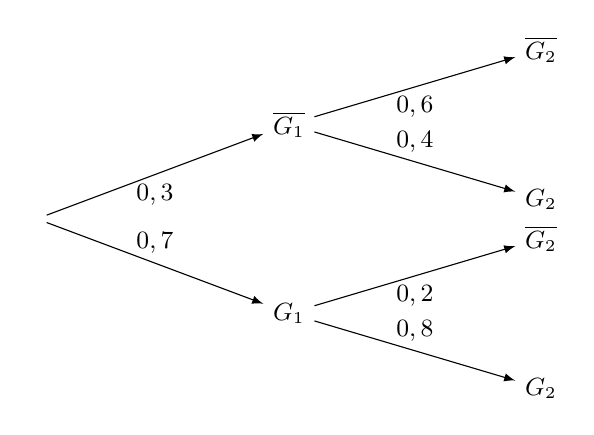
\begin{tikzpicture}[
  grow=right,
  level distance=3.2cm,
  level 1/.style={sibling distance=2.4cm},
  level 2/.style={sibling distance=1.9cm},
  edge from parent/.style={draw,-latex},
  every node/.style={font=\small}
]
\node {}
  child { node {\(G_1\)}
    child { node {\(G_2\)} edge from parent node[above] {\(0,8\)} }
    child { node {\(\overline{G_2}\)} edge from parent node[below] {\(0,2\)} }
    edge from parent node[above] {\(0,7\)}
  }
  child { node {\(\overline{G_1}\)}
    child { node {\(G_2\)} edge from parent node[above] {\(0,4\)} }
    child { node {\(\overline{G_2}\)} edge from parent node[below] {\(0,6\)} }
    edge from parent node[below] {\(0,3\)}
  };
\end{tikzpicture}
\end{center}

Parmi les probabilités suivantes, indiquer lesquelles peuvent être lues directement sur l'arbre ci-dessus ; le cas échéant, donner leur valeur.
\begin{tasks}(3)
    \task \(P(G_1)\)
    \task \(P_{G_1}(G_2)\)
    \task \(P(G_1\cap G_2)\)
    \task \(P_{\overline{G_1}}(\overline{G_2})\)
    \task \(P(G_2)\)
    \task \(P_{G_2}(G_1)\)
\end{tasks}

\end{exo}

\prof{
\begin{itemize}
    \item \(P(G_1)=0,7\) : oui, lecture directe (probabilité portée par la première branche).
    \item \(P_{G_1}(G_2)=0,8\) : oui, lecture directe (probabilité portée par une branche du second niveau).
    \item \(P(G_1\cap G_2)\) : non, cette probabilité n'est portée par aucune branche ; il faudrait utiliser la règle du produit, \(P(G_1)\times P_{G_1}(G_2)=0,7\times0,8=0,56\).
    \item \(P_{\overline{G_1}}(\overline{G_2})=0,6\) : oui, lecture directe (probabilité portée par une branche du second niveau).
    \item \(P(G_2)\) : non, cette probabilité n'apparaît sur aucune branche ; il faudrait sommer les probabilités des deux chemins menant à \(G_2\) (formule des probabilités totales, hors programme ici).
    \item \(P_{G_2}(G_1)\) : non, ce n'est pas la même quantité que \(P_{G_1}(G_2)\) ; elle ne peut pas être lue sur l'arbre (il faudrait la formule de Bayes).
\end{itemize}
}

\begin{exo}[Calculer des probas à l'aide d'un arbre][]

On reprend le contexte de l'exercice 5.

\begin{enumerate}[leftmargin=*]
    \item Calculer la probabilité \(P(U_1\cap D)\) qu'une ampoule provienne de l'usine \(U_1\) \textbf{et} soit défectueuse.
    \item Calculer de même \(P(U_2\cap D)\).
\end{enumerate}
\end{exo}

\prof{
\begin{itemize}
    \item Arbre : \(P(U_1)=0,6\) ; \(P(U_2)=0,4\) ; \(P_{U_1}(D)=0,03\) ; \(P_{U_1}(\overline D)=0,97\) ; \(P_{U_2}(D)=0,05\) ; \(P_{U_2}(\overline D)=0,95\).
    \item Seules les probabilités du deuxième niveau sont conditionnelles : \(P_{U_1}(D)=0,03\), \(P_{U_1}(\overline D)=0,97\), \(P_{U_2}(D)=0,05\), \(P_{U_2}(\overline D)=0,95\). Les probabilités du premier niveau (\(P(U_1)\), \(P(U_2)\)) ne le sont pas.
    \item \(P(U_1\cap D)=0,6\times0,03=0,018\) ; \(P(U_2\cap D)=0,4\times0,05=0,02\).
    \item On ne demande pas ici la probabilité globale qu'une ampoule soit défectueuse (\(P(D)\)) : cela nécessiterait de sommer ces deux probabilités, ce qui est la formule des probabilités totales, hors programme de cette semaine.
\end{itemize}
}

\begin{exo}[Vrai ou faux][appro]
On considère deux évènements \(A\) et \(B\) d'un univers \(\Omega\), avec \(P(A)=0,4\), \(P(B)=0,5\) et \(P(A\cap B)=0,2\). Dire si chacune des affirmations suivantes est vraie ou fausse, en justifiant.

\begin{enumerate}[leftmargin=*]
    \item \(P_A(B) = 0,5\).
    \item \(P_B(A) = 0,5\).
    \item De façon générale, pour deux évènements quelconques, \(P_A(B)=P_B(A)\).
    \item Si \(P(A)=0\), alors \(P_A(B)\) n'est pas définie.
    \item Pour deux évènements quelconques \(A\) et \(B\) avec \(P(A)\neq0\), on a toujours \(P_A(B)+P_A(\overline B)=1\).
    \item On a toujours \(P(A\cap B) = P_A(B)\times P(A)\).
\end{enumerate}
\end{exo}

\prof{
\begin{itemize}
    \item 1. Vrai : \(P_A(B)=\frac{0,2}{0,4}=0,5\).
    \item 2. Faux : \(P_B(A)=\frac{0,2}{0,5}=0,4\).
    \item 3. Faux : les questions 1 et 2 donnent déjà un contre-exemple (\(0,5\neq0,4\)).
    \item 4. Vrai : la division par \(P(A)=0\) n'est pas définie.
    \item 5. Vrai : sachant \(A\), soit \(B\) se réalise, soit \(\overline B\) se réalise, les deux évènements complémentaires \og partagent \fg{} toute la probabilité conditionnée par \(A\).
    \item 6. Vrai : c'est simplement la règle du produit, écrite dans un autre ordre.
\end{itemize}
}

\begin{exo}[D'un tableau à un arbre][]
Une entreprise de \(200\) salariés a relevé leur moyen de transport habituel selon leur lieu d'habitation.

\smallskip

\begin{center}
\begin{tabular}{|l|c|c|c|}
    \hline
     & Voiture & TC & Total \\
    \hline
    Ville & 40 & 110 & 150 \\
    \hline
    Campagne & 35 & 15 & 50 \\
    \hline
    Total & 75 & 125 & 200 \\
    \hline
\end{tabular}
\end{center}

On choisit un salarié au hasard parmi les \(200\), et on note \(V\) : \og le salarié habite en ville \fg{}, \(C\) : \og le salarié habite à la campagne \fg{} et \(T\) : \og le salarié utilise la voiture \fg{} (TC désigne \og transports en commun \fg{}, donc \(\overline{T}\) : \og le salarié utilise les TC \fg{}).

\begin{enumerate}[leftmargin=*]
    \item À l'aide du tableau, calculer toutes les probabilités nécessaires, puis recopier et compléter l'arbre pondéré ci-dessous.

    \smallskip

    \begin{center}
    \begin{tikzpicture}[
      grow=right,
      level distance=3.2cm,
      level 1/.style={sibling distance=2.4cm},
      level 2/.style={sibling distance=1.9cm},
      edge from parent/.style={draw,-latex},
      every node/.style={font=\small}
    ]
    \node {}
      child { node {\(V\)}
        child { node {\(T\)} edge from parent node[above] {\rule{1.1cm}{0.4pt}} }
        child { node {\(\overline{T}\)} edge from parent node[below] {\rule{1.1cm}{0.4pt}} }
        edge from parent node[above] {\rule{1.1cm}{0.4pt}}
      }
      child { node {\(C\)}
        child { node {\(T\)} edge from parent node[above] {\rule{1.1cm}{0.4pt}} }
        child { node {\(\overline{T}\)} edge from parent node[below] {\rule{1.1cm}{0.4pt}} }
        edge from parent node[below] {\rule{1.1cm}{0.4pt}}
      };
    \end{tikzpicture}
    \end{center}
\end{enumerate}
\end{exo}

\prof{
\begin{itemize}
    \item \(P(V)=\frac{150}{200}=0,75\) ; \(P(C)=0,25\).
    \item \(P_V(T)=\frac{40}{150}=\frac{4}{15}\approx0,27\) ; \(P_C(T)=\frac{35}{50}=0,7\).
    \item \(P_V(\overline T)=1-\frac{4}{15}=\frac{11}{15}\approx0,73\) ; \(P_C(\overline T)=0,3\).
    \item Arbre : \(P(V)=0,75\) puis branches \(\frac{4}{15}\) (\(T\)) et \(\frac{11}{15}\) (\(\overline T\)) ; \(P(C)=0,25\) puis branches \(0,7\) (\(T\)) et \(0,3\) (\(\overline T\)).
\end{itemize}
}




\begin{exo}[Tirages successifs sans remise][appro]
Une urne contient \(5\) boules rouges et \(3\) boules vertes, indiscernables au toucher. On tire au hasard une boule, on note sa couleur, on ne la remet \textbf{pas} dans l'urne, puis on tire une seconde boule.

On note \(R_1\) : \og la première boule tirée est rouge \fg{} et \(R_2\) : \og la seconde boule tirée est rouge \fg{}.

\begin{enumerate}[leftmargin=*]
    \item Calculer \(P(R_1)\).
    \item On suppose que \(R_1\) est réalisé. Combien reste-t-il de boules dans l'urne, et combien sont rouges ? En déduire \(P_{R_1}(R_2)\).
    \item On suppose maintenant que \(\overline{R_1}\) est réalisé (la première boule est verte). Déterminer de même \(P_{\overline{R_1}}(R_2)\).
    \item À l'aide de la règle du produit, calculer \(P(R_1\cap R_2)\).
\end{enumerate}
\end{exo}

\prof{
\begin{itemize}
    \item \(P(R_1)=\frac{5}{8}\).
    \item Il reste \(7\) boules dont \(4\) rouges : \(P_{R_1}(R_2)=\frac{4}{7}\).
    \item Il reste \(7\) boules dont \(5\) rouges : \(P_{\overline{R_1}}(R_2)=\frac{5}{7}\).
    \item \(P(R_1\cap R_2)=\frac{5}{8}\times\frac{4}{7}=\frac{20}{56}=\frac{5}{14}\).
    \item Remarque pour la suite : on ne demande pas ici \(P(R_2)\) (probabilité que la deuxième boule soit rouge, tout court), qui relève de la formule des probabilités totales.
\end{itemize}
}

\section{Exercices d'approfondissement : calcul littéral et probabilités}

\begin{exo}[Effectifs exprimés en fonction de \(x\)][appro]
Une association sportive propose deux activités, tennis et badminton, pratiquées par des adhérents juniors ou seniors. Le tableau ci-dessous donne les effectifs, dont certains sont exprimés en fonction d'un nombre réel \(x>0\).

\smallskip

\begin{center}
\begin{tabular}{|l|c|c|c|}
    \hline
     & Tennis & Badminton & Total \\
    \hline
    Junior & \(x\) & \(2x\) & \(3x\) \\
    \hline
    Senior & \(15\) & \(x+5\) & \(x+20\) \\
    \hline
    Total & \(x+15\) & \(3x+5\) & \(4x+20\) \\
    \hline
\end{tabular}
\end{center}

On sait que l'association compte au total \(100\) adhérents.

\begin{enumerate}[leftmargin=*]
    \item Justifier que le total général du tableau vaut \(4x+20\), puis déterminer \(x\).
    \item En déduire le tableau des effectifs, entièrement rempli avec des nombres.
    \item Calculer \(P(\text{Tennis})\) et \(P(\text{Junior}\cap\text{Badminton})\), où l'on choisit un adhérent au hasard.
    \item Calculer \(P_{\text{Junior}}(\text{Tennis})\) et \(P_{\text{Senior}}(\text{Badminton})\).
    \item Comparer \(P_{\text{Junior}}(\text{Tennis})\) et \(P_{\text{Senior}}(\text{Tennis})\). Un senior a-t-il plus tendance à jouer au tennis qu'un junior ?
\end{enumerate}
\end{exo}

\prof{
\begin{itemize}
    \item \(4x+20=100 \Rightarrow x=20\).
    \item Junior : \(20\), \(40\), total \(60\) ; Senior : \(15\), \(25\), total \(40\) ; Total : \(35\), \(65\), \(100\).
    \item \(P(\text{Tennis})=\frac{35}{100}=0,35\) ; \(P(\text{Junior}\cap\text{Badminton})=\frac{40}{100}=0,4\).
    \item \(P_{\text{Junior}}(\text{Tennis})=\frac{20}{60}=\frac{1}{3}\) ; \(P_{\text{Senior}}(\text{Badminton})=\frac{25}{40}=0,625\).
    \item \(P_{\text{Senior}}(\text{Tennis})=\frac{15}{40}=0,375 > \frac{1}{3}\approx0,333\) : un senior a (légèrement) plus tendance à jouer au tennis qu'un junior.
\end{itemize}
}

\begin{exo}[Une égalité générale][avance]
Soit \(A\) et \(B\) deux évènements d'un univers \(\Omega\), tels que \(P(A)\neq0\) et \(P(B)\neq0\).

\begin{enumerate}[leftmargin=*]
    \item Rappeler l'expression de \(P(A\cap B)\) en fonction de \(P(A)\) et \(P_A(B)\), puis en fonction de \(P(B)\) et \(P_B(A)\).
    \item En déduire l'égalité \(P(A)\times P_A(B) = P(B)\times P_B(A)\).
    \item En déduire une expression de \(P_B(A)\) en fonction de \(P(A)\), \(P(B)\) et \(P_A(B)\) uniquement.
    \item Application : \(P(A)=0,3\), \(P(B)=0,45\) et \(P_A(B)=0,6\). Calculer \(P_B(A)\).
\end{enumerate}
\end{exo}

\prof{
\begin{itemize}
    \item \(P(A\cap B)=P(A)\times P_A(B)=P(B)\times P_B(A)\) (règle du produit appliquée dans les deux sens).
    \item Les deux expressions valent \(P(A\cap B)\), d'où l'égalité.
    \item \(P_B(A) = \dfrac{P(A)\times P_A(B)}{P(B)}\).
    \item \(P_B(A)=\dfrac{0,3\times0,6}{0,45}=\dfrac{0,18}{0,45}=0,4\).
\end{itemize}
}

\begin{exo}[Résoudre une équation avec une probabilité conditionnelle][appro]
Soit \(A\) et \(B\) deux évènements avec \(P(A)=0,4\). On pose \(P_A(B)=x\) et on sait que \(P_A(\overline B)=3x-0,2\), où \(x\) est un réel de \(]0;1[\).

\begin{enumerate}[leftmargin=*]
    \item Justifier que \(x+(3x-0,2)=1\), puis résoudre cette équation.
    \item En déduire les valeurs de \(P_A(B)\) et \(P_A(\overline B)\).
    \item Calculer \(P(A\cap B)\).
\end{enumerate}
\end{exo}

\prof{
\begin{itemize}
    \item \(P_A(B)+P_A(\overline B)=1\) donc \(4x-0,2=1\), soit \(x=0,3\).
    \item \(P_A(B)=0,3\) et \(P_A(\overline B)=0,7\).
    \item \(P(A\cap B)=0,4\times0,3=0,12\).
\end{itemize}
}

\begin{exo}[Union, intersection et conditionnement][avance]
Soit \(A\) et \(B\) deux évènements d'un univers \(\Omega\). On sait que \(P(A)=x\), \(P(B)=x+0,2\), \(P(A\cup B)=0,9-x\) et \(P_A(B)=0,5\), où \(x\) est un réel de \(]0;1[\).

\begin{enumerate}[leftmargin=*]
    \item Exprimer \(P(A\cap B)\) en fonction de \(x\).
    \item En utilisant la formule \(P(A\cup B)=P(A)+P(B)-P(A\cap B)\), montrer que \(0,9-x=1,5x+0,2\).
    \item Résoudre cette équation, puis calculer les valeurs de \(P(A)\), \(P(B)\), \(P(A\cap B)\) et \(P(A\cup B)\).
    \item Vérifier que toutes ces valeurs sont bien comprises entre \(0\) et \(1\).
\end{enumerate}
\end{exo}

\prof{
\begin{itemize}
    \item \(P(A\cap B)=P(A)\times P_A(B)=0,5x\).
    \item \(P(A\cup B)=P(A)+P(B)-P(A\cap B) \Rightarrow 0,9-x = x+(x+0,2)-0,5x = 1,5x+0,2\).
    \item \(0,9-x=1,5x+0,2 \Rightarrow 0,7=2,5x \Rightarrow x=0,28\). D'où \(P(A)=0,28\), \(P(B)=0,48\), \(P(A\cap B)=0,14\), \(P(A\cup B)=0,62\).
    \item Toutes ces valeurs sont bien dans \([0;1]\), la solution est donc cohérente.
\end{itemize}
}

\begin{exo}[Cas littéral général][avance]
Soit \(A\) et \(B\) deux évènements d'un univers \(\Omega\), avec \(P(A)=p\), \(P(B)=q\) et \(P(A\cap B)=r\), où \(p\), \(q\), \(r\) sont des réels avec \(p\neq0\) et \(q\neq0\).

\begin{enumerate}[leftmargin=*]
    \item Exprimer, en fonction de \(p\), \(q\) et \(r\) uniquement : \(P_A(B)\), \(P_B(A)\), \(P(A\cup B)\), \(P(\overline A)\) et \(P_A(\overline B)\).
    \item Pourquoi doit-on nécessairement avoir \(r\leqslant p\) et \(r\leqslant q\) ?
    \item Pourquoi doit-on nécessairement avoir \(r \geqslant p+q-1\) ?
    \item En déduire un encadrement de \(r\) en fonction de \(p\) et \(q\).
\end{enumerate}
\end{exo}

\prof{
\begin{itemize}
    \item \(P_A(B)=\dfrac{r}{p}\) ; \(P_B(A)=\dfrac{r}{q}\) ; \(P(A\cup B)=p+q-r\) ; \(P(\overline A)=1-p\) ; \(P_A(\overline B)=1-\dfrac{r}{p}=\dfrac{p-r}{p}\).
    \item Car \(A\cap B\) est inclus à la fois dans \(A\) et dans \(B\) : sa probabilité ne peut pas dépasser celle de \(A\), ni celle de \(B\).
    \item Car \(P(A\cup B)=p+q-r\) est une probabilité, donc \(p+q-r\leqslant 1\).
    \item \(\max(0\,;\,p+q-1) \leqslant r \leqslant \min(p\,;\,q)\).
\end{itemize}
}

\begin{exo}[Deux chaînes de production][appro]
Une usine fabrique des smartphones sur deux chaînes de production, A et B, pour une production totale de \(1200\) appareils. On note \(x\) le nombre d'appareils fabriqués par la chaîne A (les autres proviennent de la chaîne B).

Sur la chaîne A, \(2\,\%\) des appareils sont défectueux, ce qui représente exactement \(6\) appareils défectueux.

\begin{enumerate}[leftmargin=*]
    \item En traduisant l'énoncé par une équation portant sur \(x\), déterminer le nombre d'appareils fabriqués par la chaîne A, puis par la chaîne B.
    \item On choisit un appareil au hasard parmi les \(1200\). Calculer \(P(A)\), la probabilité qu'il provienne de la chaîne A.
    \item On note \(D\) : \og l'appareil est défectueux \fg{}. Calculer \(P(A\cap D)\), puis vérifier que \(P(A)\times P_A(D)=P(A\cap D)\).
    \item Sur les \(900\) appareils de la chaîne B, on dénombre \(27\) appareils défectueux. Calculer \(P_B(D)\).
    \item Quelle chaîne de production est la plus fiable ? Justifier.
\end{enumerate}
\end{exo}

\prof{
\begin{itemize}
    \item \(2\,\%\) de \(x\) vaut \(6\) : \(0,02x=6 \Rightarrow x=300\). Chaîne A : \(300\) appareils, chaîne B : \(1200-300=900\) appareils.
    \item \(P(A)=\frac{300}{1200}=0,25\).
    \item \(P(A\cap D)=\frac{6}{1200}=0,005\). Vérification : \(P(A)\times P_A(D)=0,25\times0,02=0,005\).
    \item \(P_B(D)=\frac{27}{900}=0,03\).
    \item La chaîne A a un taux de défaut de \(2\,\%\), contre \(3\,\%\) pour la chaîne B : la chaîne A est la plus fiable.
    \item Remarque : on ne cherche pas ici le taux de défaut global de l'usine (qui nécessiterait la formule des probabilités totales).
\end{itemize}
}

\end{multicols}

\end{document}
